%% ****** Start of file template.aps ****** %
%%
%%
%%   This file is part of the APS files in the REVTeX 4 distribution.
%%   Version 4.0 of REVTeX, August 2001
%%
%%
%%   Copyright (c) 2001 The American Physical Society.
%%
%%   See the REVTeX 4 README file for restrictions and more information.
%%
%
% This is a template for producing manuscripts for use with REVTEX 4.0
% Copy this file to another name and then work on that file.
% That way, you always have this original template file to use.
%
% Group addresses by affiliation; use superscriptaddress for long
% author lists, or if there are many overlapping affiliations.
% For Phys. Rev. appearance, change preprint to twocolumn.
% Choose pra, prb, prc, prd, pre, prl, prstab, or rmp for journal
%  Add 'draft' option to mark overfull boxes with black boxes
%  Add 'showpacs' option to make PACS codes appear
\documentclass[aps,prl,twocolumn,showpacs,superscriptaddress,groupedaddress]{revtex4}  % for review and submission
%\documentclass[aps,preprint,showpacs,superscriptaddress,groupedaddress]{revtex4}  % for double-spaced preprint
\usepackage{graphicx}  % needed for figures
\usepackage{dcolumn}   % needed for some tables
\usepackage{bm}        % for math
\usepackage{amssymb}   % for math
 \usepackage{comment} % for large comment sections
\usepackage{color}
\usepackage[percent]{overpic}

\usepackage{amsmath}


% avoids incorrect hyphenation, added Nov/08 by SSR
\hyphenation{ALPGEN}
\hyphenation{EVTGEN}
\hyphenation{PYTHIA}


\begin{document}

% The following information is for internal review, please remove them for submission
\widetext
\leftline{Version 0 as of \today}
\leftline{Primary authors: Elena Gramellini}
\leftline{To be submitted to PRD.}
\leftline{Comment to {\tt elenag@fnal.gov} by xxx, yyy}
\centerline{\em LArIAT INTERNAL DOCUMENT -- NOT FOR PUBLIC DISTRIBUTION}

% the following line is for submission, including submission to the arXiv!!
%\hspace{5.2in} \mbox{Fermilab-Pub-04/xxx-E}

\title{Measurement of the ($\pi^-$, Ar) total hadronic cross section at the LArIAT experiment}
\input lariat_author_list.tex       % LArIAT authors (remove the first 3 lines
                                       % of this file prior to submission, they
                                       % contain a time stamp for the authorlist)
                                       % (includes institutions and visitors)
\date{\today}


\begin{abstract}
We present the measurement of the negative pion total hadronic cross section on Argon in the 100-1050 MeV kinetic energy range as performed at the LArIAT experiment.   Deploying a Liquid Argon Time Projection Chamber (LArTPC) in a dedicated calibration test beam line at Fermilab, LArIAT (Liquid Argon In A Testbeam) aims to experimentally calibrate this technology in a controlled environment. We use LArIAT's beamline detectors to identify candidate pions and measure their kinetic energy prior to entering the LArTPC. Once the pool of pion candidates is identified in the LAr active volume, we apply the ``thin slice method", a new technique to measure hadron-argon cross sections based on the combination of tracking and calorimetric capability of the LArTPC technology. 
Albeit our measurement of the  ($\pi^-$-Ar) total hadronic cross section is in general agreement with the predictions by the Geant4 Bertini Cascade model derived from historic measurements on lighter and heavier nuclei, a hint to a shape difference is present.
The ($\pi^-$, Ar) total cross-section has never been measured before; the outcome of this measurement will enable to quantify and reduce the systematic associated with the hadronic interaction models in neutrino-argon interactions in current and future LAr experiments such as the Short Baseline Neutrino Program and DUNE.
 



\end{abstract}

\pacs{13.15.+g Neutrino interactions, 14.40.-n	Mesons,  14.40.Be	Light mesons (S=C=B=0), 13.75.-n	Hadron-induced low- and intermediate-energy reactions and scattering (energy $le$ 10 GeV)}
\maketitle

\section{\label{sec:Motivations}Motivations}
\textcolor{red}{Need to define signal}
Motivations: existing measurements + interpolation between heavier and lighter nuclei
Methods used in other measurements (concise)
Historic measurements of hadronic cross sections are performed on thin targets [\textcolor{red}{A CIT is needed here}]. At their core, these experiments consists in shooting a beam of particles with a known flux on a thin slab of material and recording the outgoing flux, under the assumption that the target centers are uniformly distributed in the material and that no center of interaction sits in front of another. 


\section{\label{sec:ExperimentalSetup}Experimental Setup}
We briefly describe here the features and use of the LArIAT beamline detectors and LArTPC  relevant to the cross section measurement; we refer the reader to [\textcolor{red}{cit detector paper}] for a detailed description of LArIAT's experimental setup.

\subsection{\label{sec:Beamline}Beamline} 
\begin{figure*}
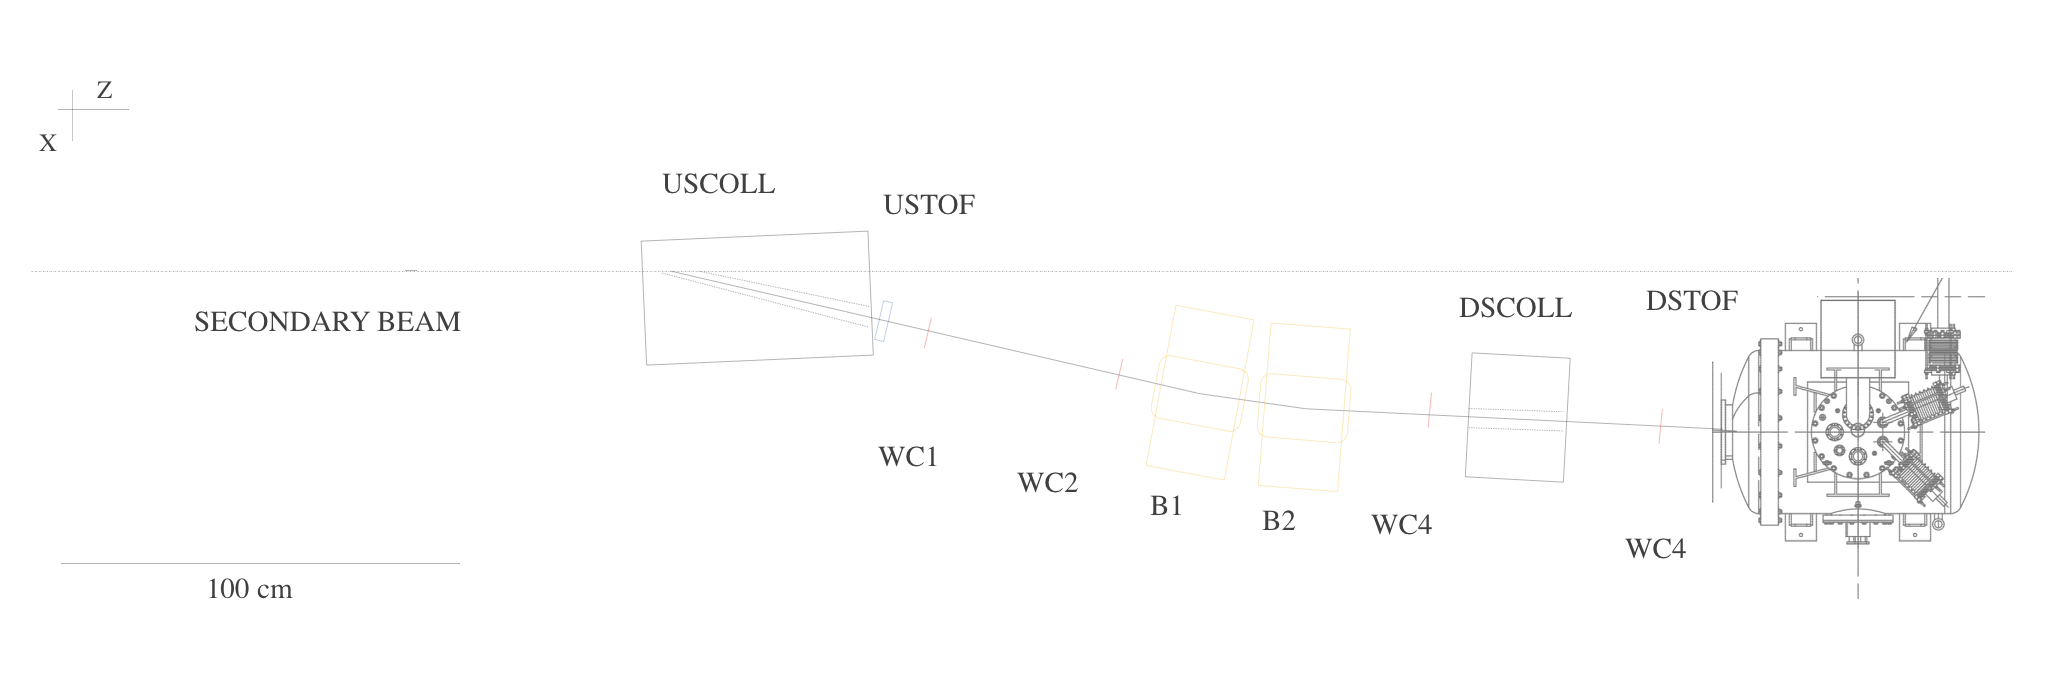
\includegraphics[width=\textwidth,height=\textheight,keepaspectratio]{Tertiary.png}
 \put (-500,185) {\huge \textcolor{red}{Needs WORK}}
\caption{Bird's eye view of the LArIAT tertiary beamline. In grey: upstream and downstream collimators; in yellow: bending magnets; in red: multi wire proportional chambers; in blue: time of flight; in green: liquid argon TPC volume; in maroon: muon range statck.}
\label{fig:beamlinebird}
\end{figure*}


%\begin{overpic}[width=0.5\textwidth,grid,tics=10]{momentumPiMuE.png}
% \put (20,85) {\huge$\displaystyle\gamma$}
%\end{overpic}


Scope of the LArIAT beamline instrumentation is to identify the particle type and measure the momentum of the particles entering the LArIAT TPC. Figure \ref{fig:beamlinebird} shows a bird's eye view of the LArIAT tertiary beamline where we highlighted the key components for the cross section measurement:  two bending electromagnets (yellow), a set of four wire chambers (red) and two time-of-flight scintillating paddles (blue).  The magnets' polarity determines the charge of the particles selected in the tertiary beam: running the magnets in negative polarity selects negatively charged particles. The strength for the magnetic field is set by the amplitude of the current in the magnets. For this work,  the current settings explored were -60A (B $\sim$0.21 T) and -100A (B $\sim$0.35 T).  The combination of magnets and wire chambers forms the LArIAT spectrometer which measures the particles' momentum at the fourth wire chamber, $p_{\text{Beam}}$, with a relative uncertainty of 2\%. Figure \ref{fig:momentum} shows the distribution of  $p_{\text{Beam}}$ for the Run II negative polarity data used in this work, which spans from $\sim200$ to $\sim1200$ MeV/c. 
%\begin{comment}     
\begin{figure}
  \centering  
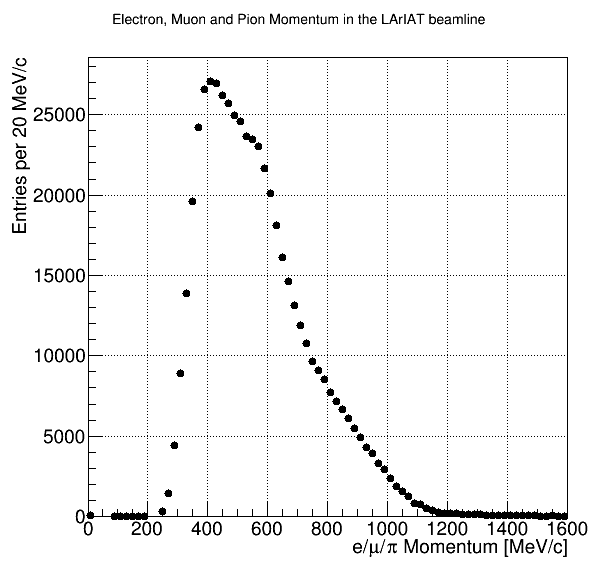
\includegraphics[width =0.4\textwidth]{momentumPiMuE.png}
\caption{Momentum spectrum in the LArIAT beamline  for Run II negative polarity data.}
\label{fig:momentum}
\end{figure}



We leverage the measurement of the momentum in conjunction with the measurement of the time of flight to calculate the particle's invariant mass $m_{\text{Beam}}$ as 
\begin{equation}
m_{\text{Beam}} = \frac{p_{\text{Beam}}}{c}\sqrt{\biggl(\frac{TOF*c}{l}\biggr)^2 -1},
\label{eq:mass}
\end{equation}
 where $c$ is the speed of light and $l$ is the length of the particle's trajectory between the time of flight paddles. 





Figure \ref{fig:mass} shows the distribution of the invariant mass for the Run II negative polarity runs. We classify beamline events into the different categories as follows:

\begin{tabular}{lllrl}
& & & &\\
 $\pi/\mu/e$: &                               & $m_{\text{Beam}}<$& 350~MeV/c$^2$&\\
 kaon:           & 350~MeV/c$^2 <$ & $m_{\text{Beam}}<$& 650~MeV/c$^2$&\\
 antiproton:   & 650~MeV/c$^2 <$ & $m_{\text{Beam}}<$& 3000~MeV/c$^2$&.\\
& & & &\\
\end{tabular}


%\begin{itemize}
%\item[-] $\pi/\mu/e$:  $m_{\text{Beam}}<$ 350~MeV/c$^2$
%\item[-] kaon: 350~MeV $< m_{\text{Beam}} <$ 650~MeV/c$^2$
%\item[-] antiproton: 650~MeV $<m_{\text{Beam}}<$ 3000~MeV/c$^2$.
%\end{itemize}

It should be noted that pions are the main component of the LArIAT beam of charged particle and that the sole use of the aforementioned beamline instrumentation does not allow to discriminated between electrons, muons and pions. We make use of the topological difference in the LArTPC between track and electromagnetic shower to mitigate the presence of electrons in the pion sample. A small contamination of electrons and muons still remains, which we account for as beamline background in the cross section measurement.

%\begin{comment}     
\begin{figure}
  \centering  
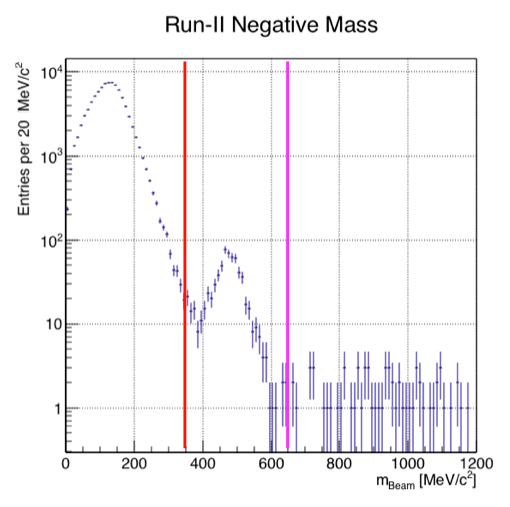
\includegraphics[width =0.4\textwidth]{massRunII.png}
\caption{Distribution of the beamline mass as calculated according to equation \ref{eq:mass} for the Run-II events reconstructed in the beamline, negative polarity runs. The classification of the events into $\pi^-/ \mu^-/e^-$, K$^-$, or antiproton is based on these distributions, whose selection values are represented by the vertical colored lines.}
\label{fig:mass}
\end{figure}


\subsection{\label{sec:LArTPC}LArTPC}

The LArIAT LArTPC is a box of dimensions 47 cm (drift) by 40 cm (height) by 90 cm (depth) equipped with an  electric field of 490 V/cm. LArIAT induction and collection planes consist of 240 wires each at 4 mm spacing. The wires are oriented at +/- $60^{\circ}$ from the vertical direction, while the beam direction is oriented 3 degrees off the $z$ axis in the $XZ$ plane.   Beamline particles enter the TPC roughly at the center of the front face leaving traces of ionization the in TPC. The ionization signals on the wires are then recorded by the LArIAT DAQ, stored and processed offline. LArIAT makes use of the LArSoft toolkit \cite{EricFChurck} for data acquisition, signal processing, event reconstruction and TPC simulation. 

The processing and reconstruction chain of the TPC signals, from the pulses on the sense wire to the construction of three dimensional objects with associated calorimetry can be summarized in the following categories: \emph{Deconvolution}, \emph{Hit Reconstruction}, \emph{2D Clustering}, \emph{3D Tracking}, \emph{Calorimetry Reconstruction}. \\ %A visualization of the signal processing workflow is shown in figure \ref{fig:SignalProc}.\\

%\begin{figure*}[hbpt]
%\centering
%\includegraphics[width=\textwidth]{SignalProc.jpg}
%\caption{A scheme of a typical signal processing workflow in LArSoft.}
%\label{fig:SignalProc}
%\end{figure*}

\textbf{Deconvolution.} Induction and collection planes have different field responses, given the different nature of the signals on these planes: the wires on the induction planes see the inductive signal of the drifting charge, while the wires on the collection planes see the current derived from the charge entering the conductor. Thus, signals on the induction plane are bipolar pulses and signal on the collection plane are unipolar pulses. %, see Figure \ref{fig:SignalProc} panel a). 
The first step in signal processing is deconvolution, that is a series of off-line algorithms geared towards undoing the detector effects. The result of the deconvolution step is  the production of  a comparable set waveforms on all planes presenting unipolar, approximately gaussian-like pulses. % (Figure \ref{fig:SignalProc} panel b). 
Signal from all planes are treated on equal footage beyond this point.\\


\textbf{Hit Reconstruction.} The second stage of the signal processing is the reconstruction of hits, indicating an energy deposition in the detector.  A peak finder scans the deconvolved TPC waveforms for each wire on the whole readout time looking for spikes  above  the waveform's baseline. It then fits these peaks with gaussian shapes and stores the fit parameters such as the quality of the fit, the peak time, height and area under the gaussian fit. The information resulting from this process on a single spike form a single reconstructed ``hit". %, see Figure \ref{fig:SignalProc} panel c).
 The next steps in the event reconstruction chain will then decide which hits to use according to their goodness of fit. %It is important to notice how the height and width of the hit depend on the topology of the event: for example, a particle running  parallel to the wire planes will leave a series of narrow individual hits, one on each consecutive wire, while a particle traveling towards the planes will leave long, wide hits on very few wires. 
The height of the hits and their integral is proportional to the charge collected on the wire.
The event reconstruction chain uses collections of hits to form more complex objects associated with the particles in the detector. The development of different approaches to accomplish this task is an extremely hot topic in LArTPC event reconstruction which spans from more traditional approaches such as line-clustering  \cite{Barker2011} to the use of machine learning tools \cite{1748-0221-12-03-P03011}. Generally speaking, the scope of hit clustering and event reconstruction is to provide shower-like or track like-objects with an associated energy reconstruction. This is because different particles have different topology in the detector -- electrons and photon create electromagnetic showers,  resulting in shower-like topologies, while muons and hadrons  leave track-like signals.  For the scope of this work, we will describe only LArIAT's approach to track reconstruction even if we recognize that the breath of LArTPC event reconstruction is much wider. We are interested in the reconstruction of pions in the active volume, whose topology is track-like.\\

\textbf{2D Clustering Reconstruction.} 
The LArIAT reconstruction of track-like objects starts by clustering hits on the collection and induction planes separately with the use of the TrajCluster clustering package\cite{Baller2016}. 
TrajCluster looks for a collection of hits in the wire-time 2D space which can be described with a line-like 2D trajectory. TrajCluster reconstructs trajectories by adding trajectory points to the leading edge of the trajectory while stepping through the 2D space of hits. Several factors determine whether a hit is added to the trajectory, including but not limited to the goodness of the fit of the single hit, the charge of the hit compared to the average charge and RMS of the hits already forming the trajectory, the goodness of trajectory fit with and without the hit addition, the angle between the two lines formed by the collection of hits before and after the considered hit in the trajectory.
The final product of this reconstruction stage is the collection of bidimensional clusters on each wire plane.\\%, see Figure \ref{fig:SignalProc} panel d).\\

\textbf{3D Tracking.} The 3D tracking set of algorithms uses clusters close in time on the induction and collection planes as starting point to form a 3D track. Firstly, it constructs a tentative 3D trajectory using the edges of the clusters. Then, it  projects back the tentative trajectory on to the planes and adjusts the parameters of the 3D track fit such that they minimize the distance between the fit projections and the track hits in all wire planes simultaneously.  Tridimensional tracking can use multiple clusters in one plane, but it can never break them into smaller groups of hits. This algorithm was first developed for the ICARUS collaboration\cite{Antonello2013}. The final product of this reconstruction stage is the formation of  tridimensional objects in the TPC active volume.\\%, see Figure \ref{fig:SignalProc} panel e).\\

\textbf{Calorimetry.} The last step in the event reconstruction chain is to assign calorimetric information to the track objects. Calorimetry is performed separately on the different planes. A multi-step procedure is needed to retrieve the energy deposited in the TPC  from the charge seen by the wires.
For each hit associated with the track object, the calorimetry set of algorithms calculates the charge seen on every wire integrating the area underneath the gaussian fit; then, it corrects this raw charge by the electron life time, the electronic noise on the considered wire and the recombination effect. Lastly an overall calibration of the energy is applied and the calorimetric information for the given track is assigned. \\

Signal processing and event reconstruction provide the collection of TPC tracks per event and their associated tracking and calorimetric information. We use the reconstructed track direction and position at the front face of the TPC to match one TPC track to the beamline candidate. We reject events with either zero or multiple matches. In an effort to reduce electron contamination, we filter events based on their topology in the TPC: if more than 5 short tracks (track length $<$ 10 cm) are present in the proximity of the matched TPC track, the event is classified as electron and rejected. The calorimetry information entails the measurement of the energy deposited $E_{\text{Dep},i}$ along the pion's path at every ``track pitch", i.e. at every segment between two 3D points of the trajectory. The track pitch distribution is shown in Figure \ref{fig:pitch}; for both data and simulation, the track pitch averages at $\delta {\emph{X}}$ = 4 mm/(sin($60^{\circ}$)cos($3^{\circ}$)) $\approx$ 4.7~mm. 
The energy deposited $E_{\text{Dep},i}$, whose distribution is shown in \ref{fig:enDep}, is obtained from the signals on the collection plane.  This information is leveraged together with the measurement of the beamline momentum to assess the kinetic energy of the matched pion candidate at each point of the pion reconstructed track. We start by estimating the pion's  kinetic energy at the TPC front face, $ E^{kin}_{\text{Front Face}}$, as 
\begin{equation}
 E^{kin}_{\text{Front Face}}  = \sqrt{p^2_{\text{Beam}} - m^2_{\text{Beam}}} - m_{\text{Beam}} - E_{\text{Loss}},
\label{eq:enFF}
\end{equation}
where $p_{\text{Beam}}$ is the momentum measured by the LArIAT spectrometer, $m_{\text{Beam}} = 139.57018\pm0.00035$ MeV is the pion mass [\textcolor{red}{cite pdg}], $E_{\text{Loss}}$ is a correction for the kinetic energy lost in the un-instrumented material between the beamline and the TPC front face. Figure \ref{fig:ELoss100A} shows the $E_{\text{Loss}}$ distribution for the simulation of the -100A Run II data. To obtain the kinetic energy at each point of the pion reconstructed track, we iteratively subtract the measurement of the energy deposited $E_{\text{Dep},i}$ from $ E^{kin}_{\text{Front Face}}$; in formulae, the kinetic energy at the $j^{th}$ point of the track  $E_{j}^{kin}$ is given by
\begin{equation}
 E_{j}^{kin} =  E^{kin}_{Front Face} - \sum_{i < j} E_{\text{Dep},i}.
\label{eq:KEj}
\end{equation}

The finely grained measurement of the kinetic energy, possible only thanks to the combination of tracking and calorimetry of the LArTPC, represents foundation of the thin slice method discussed below.\\

\begin{figure}
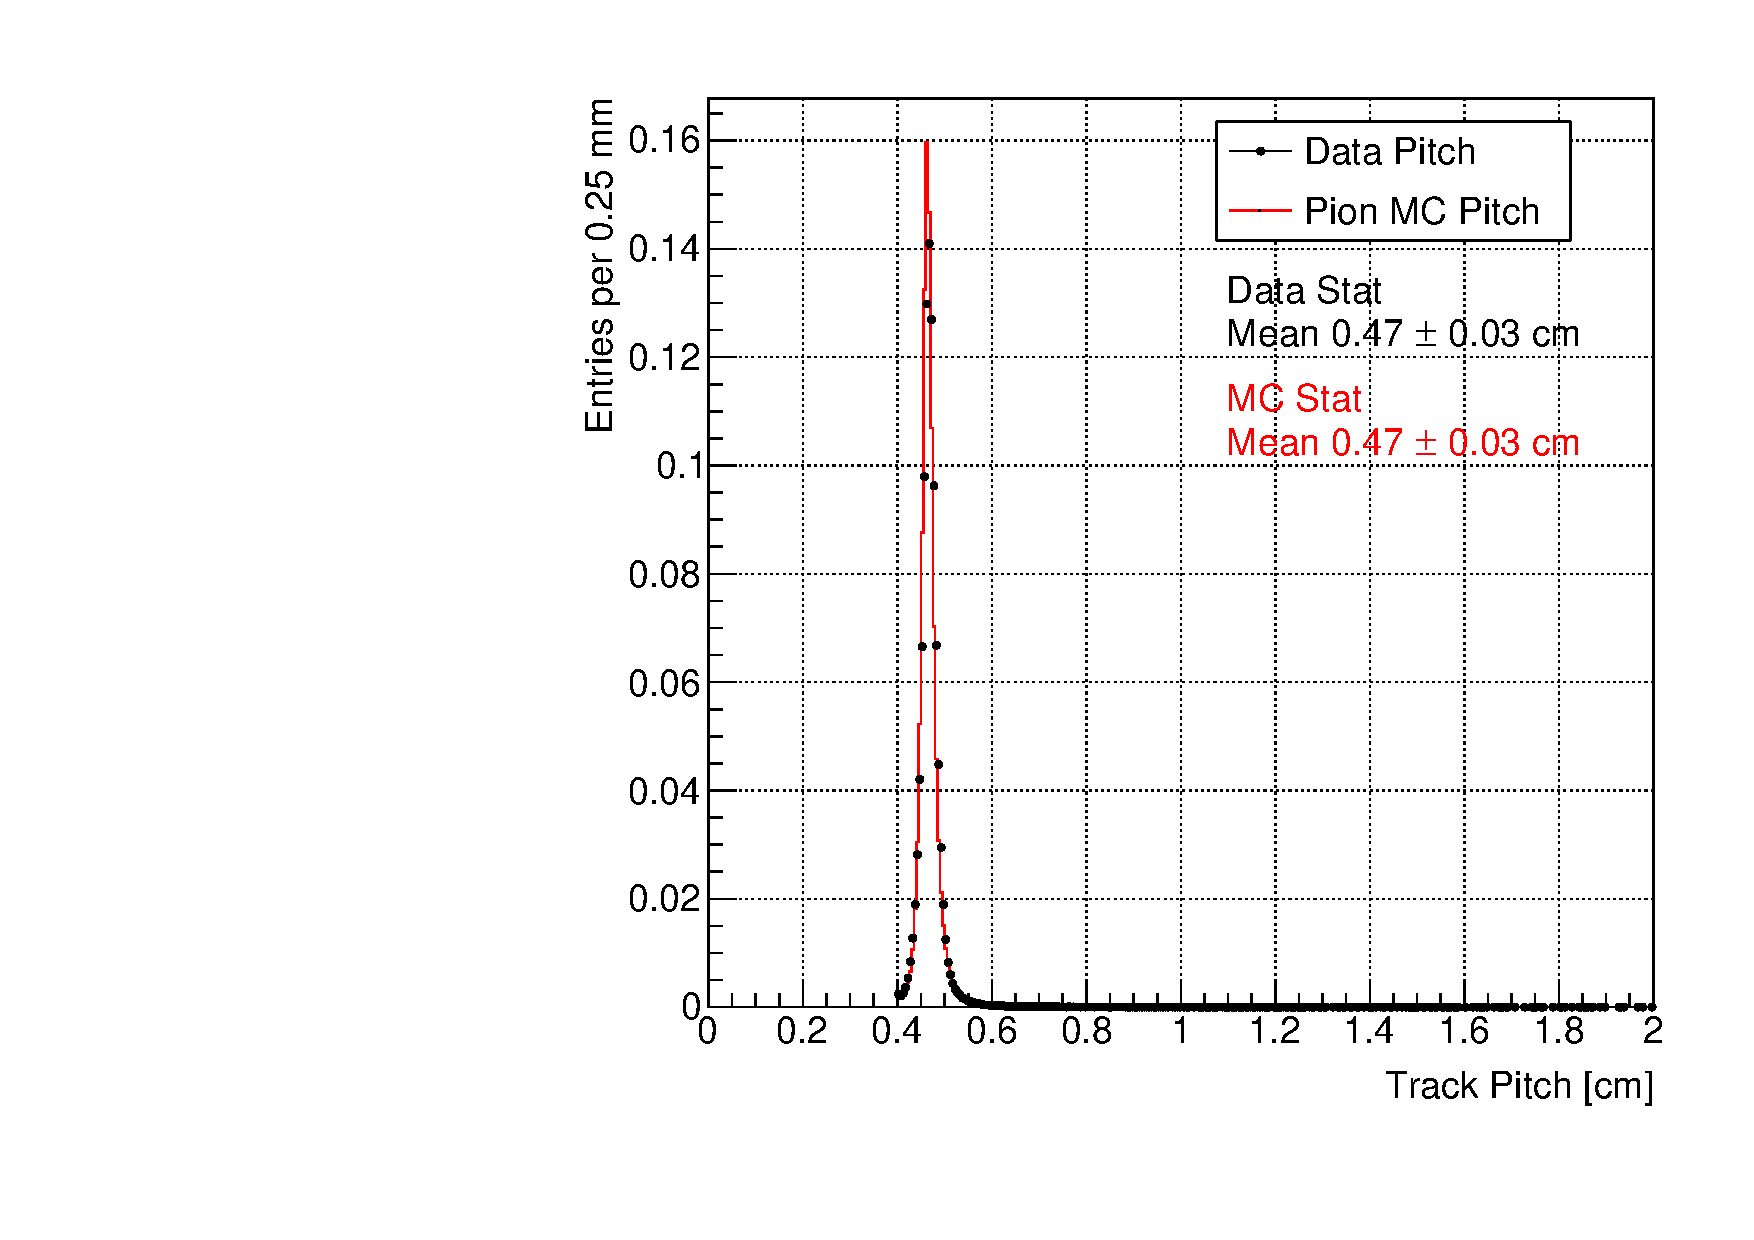
\includegraphics[width =0.4\textwidth ]{PitchPi}
\caption{\label{fig:pitch}  Pitch distribution for the Run II negative polarity data displayed in black, MC in red.}
\end{figure}
\begin{figure}
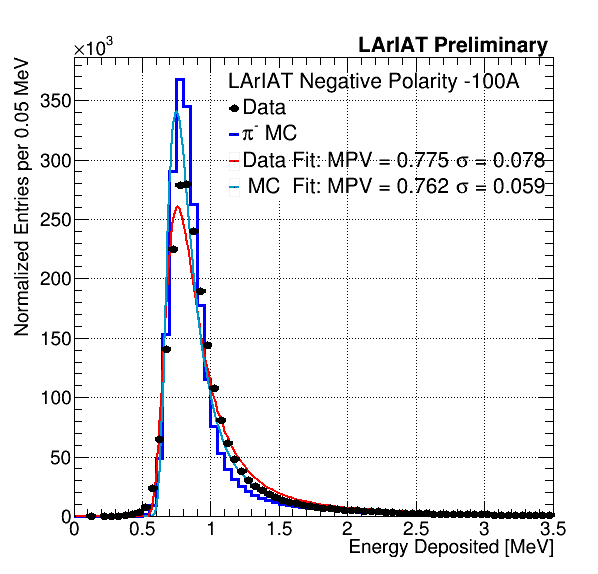
\includegraphics[width =0.4\textwidth ]{DepEnergy_Fit_v4100A.png}
\caption{\label{fig:enDep}  Energy deposition distribution for Run II negative polarity data at -100A magnet configuration displayed in black, MC in red.}
\end{figure}

\begin{figure}
\centering
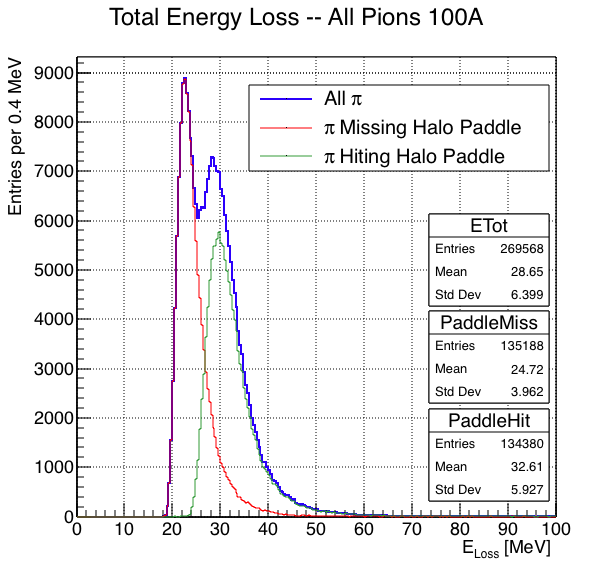
\includegraphics[width=0.45\textwidth]{E_loss100A.png}
\caption{\label{fig:ELoss100A}  True energy loss between WC4 and the TPC front face according to the MC simulation of negative polarity data at -100A. Two populations are visible, depending on the uninstrumented material seen by the beamline pion: the distribution for the pions missing the halo scintillation material is shown in red, and the distribution for the pions hitting the halo is shown in green, the distribution for the whole data sample is shown in blue.  }
\end{figure}



\subsection{\label{sec:Simulation}Simulation}
The LArIAT simulation toolkit used in this work is a combination of two Monte Carlo simulations: the G4Beamline Monte Carlo  [\textcolor{red}{cit needed}] and the Data Driven single particle Monte Carlo (DDMC).  G4Beamline simulates the beam collision at the LArIAT target, the energy deposited by the particles in the beamline detectors, and the action of the magnets, effectively accounting for particle transportation through the beamline from the LArIAT target until the LArTPC. G4Beamline accounts for the beamline trigger and simulates the particle's composition in the beam. G4Beamline provides the relative percentages of particle species which the DDMC simulates downstream from the fourth wire chamber into the cryostat and into the LArTPC.  The measurement of the beamline particles' momentum and position at the fourth wire chamber performed on data serves as a basis for the DDMC event generation: the DDMC simulation samples from the joint distribution of the data momentum and position using a 5-dimensional hit-or-miss sampling procedure. This sampling generates MC events  with the same momentum and position distributions as data, with the additional benefit of accounting for the correlations between them. A LArSoft simulation module launches single particle MC from the location of the fourth wire chamber (100 cm upstream to the LArTPC) using the generated events. The particles are free to decay and interact in their path to the LArTPC according to the Geant4 simulation. We use the DDMC samples in several occasions: to propagate the estimated beamline background to the pion cross section, to calibrate the energy loss upstream of the LArTPC,  and to study the tracking and the calorimetric performance  in the LArTPC. 


\subsection{\label{sec:EventSelection}Beamline Event Selection}
\begin{table}
\caption{\label{tab:MCafterCutContaminants}Expected beamline composition for events selected in.}
\begin{ruledtabular}
\begin{tabular}{ l | l | l | l | l | l | l  |}
 &  \multicolumn{3}{c|}{I$_{\text{Magnets}} =$ -60A} & \multicolumn{3}{c|}{I$_{\text{Magnets}} =$ -100 A }\\
& MC $\pi$   & MC  $ \mu$ & MC  $e$ & MC  $\pi$ & MC  $\mu$ & MC  $e$  \\
\hline
&  &  &  & & &\\  
Expected &  &  &  & & &\\  
Composition&  88.5\%   & 8.2\%   & 3.3 \%   & 94.0\%	& 5.3\% & 0.7\%\\
in XS sample               &                      &                       &                   &                       &                        &\\  
&                      &                       &                   &                       &                        &\\  
\end{tabular}
\end{ruledtabular}
\end{table}

In data, the selection of beamline events proceeds as follows; we first reconstruct the beamline event, checking that the particle trajectory is plausible, which means rejecting events whose trajectory crosses impenetrable material in the beamline, such that the magnets' steel. We select beamline events whose beamline momentum is greater than 420 MeV/c, so to minimize the occurrence of a pion capturing or decaying inside the chamber.  For each the negative polarity Run II events classified as $\pi/\mu/e$, we check the number of TPC tracks in the front portion of the TPC: in case more than four tracks are present in the first 14 cm we reject the event,  since the pile up of beam particles would affect the precision of the track reconstruction.
The events that are matched to a TPC track and that survive the shower filter form the pool of beamline events for the cross section analysis. This pool is made of 40841 beamline pion candidates in data. 

In simulation, G4Beamline estimates the beam composition at the fourth wire chamber used to weight the number of electrons, muons and pions simulated with the DDMC. The simulated beamline events undergo the same selection flow as data: Table \ref{tab:MCafterCutContaminants} shows the predicted percentage of pion, muons and electrons in the pion beamline candidates selection. We feed beamline candidates the ``thin slice method" machinery in order to measure the negative pion total hadronic cross section. 




\begin{table}
\caption{\label{tab:beamlineDataSelection}Selection flow on the number of data events for Run-II Negative polarity towards the definition of beamline events for the pion cross section measurement.}
\begin{ruledtabular}
\begin{tabular}{l|r}
                                                        &  N Beamline Events     \\ \hline
Events Reconstructed in Beamline        &  158396     \\ \hline
Plausible Trajectory \& $p_{\text{Beam}}$ selection       &   147468    \\ \hline
Beamline $\pi^-/\mu^-/e^-$  Candidate  &   138481    \\ \hline
Events Surviving Pile Up Filter              &   108929    \\ \hline
Events with TPC Match                         &    41757     \\ \hline
Events Surviving Shower Filter             &    40841     \\ 
\end{tabular}
\end{ruledtabular}
\end{table}



\section{\label{sec:ThinSliceMethod}Thin Slice Method}
The pion interaction probability $P_{\text{Int}}$ in an argon target of thickness $\delta X$  is related to the cross section $\sigma_{\text{TOT}}$ by the following equation, 
\begin{equation}
P_{\text{Int}} = 1- e^{-\sigma_{\text{TOT}}\text{ } n \text{ }\delta X}
\label{eq:thinTargetXS}
\end{equation}
where $n$ is the density of the target centers, $n$. In an experiment where a beam of pions is incident on the target, the interaction probability $P_{\text{Int}}$ can be statistically estimated as the ratio between the number of pions interacting in the thin target $N_{\text{Int}}$ (interacting flux) and the number of incident pions $N_{\text{Inc}}$ (incident flux). 
If the interaction length is significantly longer than the width of the target, i.e $\lambda_{\text{Int}} \gg \delta X$, we can assume that the target centers are uniformly distributed in the material and that no center of interaction sits in front of another -- the thin target approximation. In this case, it is possible to find a simple proportionality relationship between the cross section and the interaction probability by a Taylor expansion of the exponential function:
 \begin{equation}
 \sigma_{\text{TOT}}  = \frac{1}{n \text{ }\delta X}\frac{N_{\text{Int}}}{N_{\text{Inc}}}.
\label{eq:thinTargetXSSolved}
\end{equation}



Since the expected interaction length of pions in liquid argon is of the order of $\lambda_{\text{Int}} \sim 50$ cm [\textcolor{red}{A CIT is needed here}], the LArIAT TPC and its 90 cm of depth are not a thin target. However, the granularity of the LArIAT LArTPC allows us to assess the presence of a pion and to measure its kinetic energy approximately every 4.7~mm along its trajectory in the detector's active volume. We can thus treat the argon volume as a sequence of many adjacent thin targets, recovering the thin target approximation in each slice of argon. 


We consider each slice of argon {\emph{j}} an independent thin target experiment for which the incoming pion has a kinetic energy of  $E^{kin}_j$, measured according to equation \ref{eq:KEj}. It should be noticed that each beamline pion candidate is likely to traverse multiple slices, thus participating in multiple independent thin target experiments.   We apply the cross section calculation from Equation~\ref{eq:thinTargetXSSolved} in bins of kinetic energy: if a pion of kinetic energy $E^{kin}_j$ enters a slice, it contributes to the incident flux at the energy bin corresponding to $E^{kin}_j$.  Within the slice, the pion may or may not interact. If it does, it also contributes to the interacting flux at the same energy bin. If the pion does not interact,  it will enter the next slice and the evaluation of the fluxes is repeated for the new kinetic energy $E^{kin}_{j+1}$. The pion decreases its kinetic energy in its path within the TPC due to ionization and excitation of the argon; thus, for the same beamline pion candidate, slices close to the TPC front face correspond to higher $E^{kin}_j$ compared to slices close to the TPC back face. We evaluate the incident and interacting fluxes for all the beamline pion candidates in the selected sample.  %The cross section as a function of kinetic energy, $\sigma_{TOT}( E^{kin})$ is then evaluated to be proportional to the ratio $\frac{N_{\text{Int}}( E^{kin})}{N_{\text{Inc}}( E^{kin})}$ -- bin by bin ratio. 

Since our goal is to measure the total interaction cross section independently  from the topology of the interaction, we determine that a pion interacted simply by requiring that the last point TPC track lies within the fiducial volume (FV), i.e. the volume contained within 1 cm from the TPC walls in the drift and vertical directions, 1 cm from the TPC front face and 4 cm from the TPC back face.
If the TPC track crosses the boundaries of the FV, the track is considered ``through going", no interaction point is found and no point external to the FV is consider for the fluxes evaluation. 


%\textcolor{red}{inefficiency and background}

%The only slices traversed by the pion beamline candidate track considered to fill the  $N_{\text{Int}}$ and  $N_{\text{Inc}}$ distributions are the ones contained in the fiducial volume. 
 
% A notable background pertinent only to the $N_{\text{Int}}$  distribution are cases in which the hadrons decays inside the TPC. In those cases in fact, the tracking ends inside the TPC but the interaction is not hadronic. The handling of decay background is treated in a slightly different way for the pion and kaon section, details can be found in sections \ref{ch:PionXSBkgSub} and \ref{ch:KaonXSRaw} respectively.


%\subsection{\label{sec:RawXS}Raw Cross Section}
\subsection{\label{sec:Corrections}Fluxes Corrections}
In the evaluation of the interacting and incident fluxes as a function of the pion kinetic energy,  two caveats are in place: a) residual muons and electrons are present in the beamline pion sample, b) TPC event reconstruction affects the evaluation of  $N_{\text{Int}}$ and $N_{\text{Inc}}$.
We then need to repackage Equation~\ref{eq:thinTargetXSSolved} at kinetic energy $E^{kin}_i$, as a function of the measured fluxes in data $N^{\text{Data}}_{\text{Int}}$ and $N^{\text{Data}}_{\text{Inc}}$, the corresponding beamline background $B^{ \text{Int}}$ and $B^{ \text{Inc}}$ and corrections for reconstruction effects $\epsilon^{\text{Int}}$ and $\epsilon^{\text{Inc}}$ as follows

\begin{equation}
 \sigma^{\pi^-}_{TOT}(E^{kin}_i) = \frac{1}{n \text{ }\delta X}\frac{ \epsilon^{\text{Inc}}_i [ N^{ \text{Data}}_{ \text{Int,i}} - B^{ \text{Int}}_i] }{   \epsilon^{\text{Int}}_i [N^{ \text{Data}}_{ \text{Inc,i}} - B^{ \text{Inc}} _i]},
\label{eq:True}
\end{equation}
where the subscript $i$ highlights that the quantities are evaluated separately in each kinetic energy bin.\\



\textbf{Corrections for Reconstruction Effects.}
We rely on the capacity of the tracking algorithm to identify the incoming pion in the TPC and to stop the tracking at the interaction point, evaluating whether or not the pion interacted.  The tracking algorithm has an intrinsic limitation in resolving shallow scattering angles, effectively determining a selection on the distribution of the scattering angle of hadronic interaction entering the cross section measurement.  Since we assess interaction angles smaller than 5 deg to be indistinguishable for the reconstruction, we limit our ability to measure the cross section for interaction angles greater than 5.0 deg. 

The interacting flux depends on the efficiency of the tracking of finding the pion in the TPC and of finding the interaction point. It should be noted that the incident flux also depends on the same tracking efficiencies, albeit in a different way. If the tracking does not stop at an interaction point but keeps adding subsequent points to the pion trajectory, the missed interaction constitutes an inefficiency for the interaction flux and the slices corresponding to the extra trajectory points result in a background for the incident flux. On the contrary, if the tracking stops before an interaction point,  that flagged interaction point constitues a background for the interaction flux and the missed subsequent slices represent an inefficiency for the incident flux. We encode both the inefficiency and background due to the reconstruction of the pion track in the flux corrections $\epsilon^{\text{Int}}_i$ and $\epsilon^{\text{Inc}}_i$. We use a sample of DDMC pions to evaluate the flux corrections as follows,

\begin{equation}
 \epsilon^{\text{Int}}_i  =  \frac{N^{\text{ Reco MC $\pi$}}_{\text{Int,i}}}{ N^{\text{ True MC  $\pi$}}_{\text{Int,i}}  } \hspace{0.5cm}\text{and}\hspace{0.5cm}  \epsilon^{\text{Inc}}_i  =  \frac{N^{\text{ Reco MC $\pi$}}_{\text{Inc,i}}}{ N^{\text{ True MC  $\pi$}}_{\text{Inc,i}}  },
\end{equation}

where $N^{\text{ True MC  $\pi$}}_{\text{Int,i}}$ is the expected number of interacting pions at the kinetic energy $E^{kin}_i$ according to the \textcolor{red}{ cross check these} Geant4 10.03.p1 FTFP\_BERT interaction model and  $N^{\text{ Reco MC $\pi$}}_{\text{Int,i}}$ is the number of reconstructed interacting pions at the same kinetic energy; analogous definitions apply to the correction on the incident flux. \\




\textbf{Corrections for Beamline Background.}
Even if pions are by far the biggest beam component in selected beamline candidates, residual muons and electrons are present in the sample. We estimate the muon and electron contributions to the incident and interacting flux vin data ia MC. Our goal is to estimate  $B^{ \text{Int}}_i$ and  $B^{ \text{Inc}}_i$ , i.e. the number of non-pion entries in the interacting and incident flux at each kinetic energy bin $E^{kin}_i$ in the range of the cross section measurement. The estimated percentages of muons, $w_\mu$,  and electrons, $w_e$,  in the sample of pion beamline candidates are reported in Table \ref{tab:MCafterCutContaminants}. We estimate 
$B^{ \text{Int}}_i$ to be

\begin{equation} \label{eq:Contaminants}
\begin{split}
B^{ \text{Int}}_i & = M^{ \text{Int}}_i + E^{ \text{Int}}_i \\
                         & =  \frac{w_\mu P^{Data}}{P^{MC}_\mu} M^{MC}_{ \text{Int,i}} + \frac{w_e P^{Data}}{P^{MC}_e}E^{MC}_{ \text{Int,i}},
\end{split}
\end{equation}


where $M^{ \text{Int}}_i$ and $E^{ \text{Int}}_i$ are the estimated muon and electron contributions to the the interacting flux at the kinetic energy bin $E^{kin}_i$ for data, $P^{Data}$ is the total number of beamline pion candidates in data, $P^{MC}_\mu$ and $P^{MC}_e$ are the number of MC beamline muons and electrons, $M^{MC}_{ \text{Int,i}}$ and $E^{MC}_{ \text{Int,i}} $ are  the MC muons and electrons contributions to the interacting flux in MC at kinetic energy bin $E^{kin}_i$.\\
Analogous definition hold true for the incident flux. We estimate $M^{MC}_{ \text{Int,i}}$, $M^{MC}_{ \text{Inc,i}}$  $E^{MC}_{ \text{Int,i}} $, and $E^{MC}_{ \text{Inc,i}} $ by shooting  DDMC samples of muons and electrons in the TPC and applying the thin slice method to the selected MC beamline candidates.


\subsection{\label{sec:Corrections}Treatment of the uncertainties}

\section{\label{sec:Results}Result}
% sections are not used for PRL papers
The top plot of Figure \ref{fig:epsart} shows the measurement of the ($\pi^-$-Ar) total hadronic cross section,  for  scattering angles greater than 5$^\circ$, as the result of the fluxes' corrections and combination of the 60A and 100A data sets. The statistical uncertainty and the sum in quadrature of statistical and systematic uncertainty are shown in black;  the FTFP\_BERT Geant4 prediction for the total hadronic cross section for angle scattering greater than 5$^\circ$ is displayed in green. 
With the exception of the highest energy bins (energy greater than 800 MeV), the systematic uncertainties are the dominant uncertainties; the lion's share of the systematic uncertainty results from our uncertainty on the beam composition. The bottom panel of Figure  \ref{fig:epsart} shows the relative deviation between the measured cross section and the FTFP\_BERT  Geant4 predicted cross section.
\textcolor{red}{Considerations about agreement and disagreements}

Table \ref{tab:XSsummary} summarizes the cross section as a function of kinetic energy and  the associated total uncertainty; it also reports the fluxes corrected by the beamline background for the 60A and 100A sample and the corresponding corrections due to the reconstruction of the pion track.\\


\begin{figure}
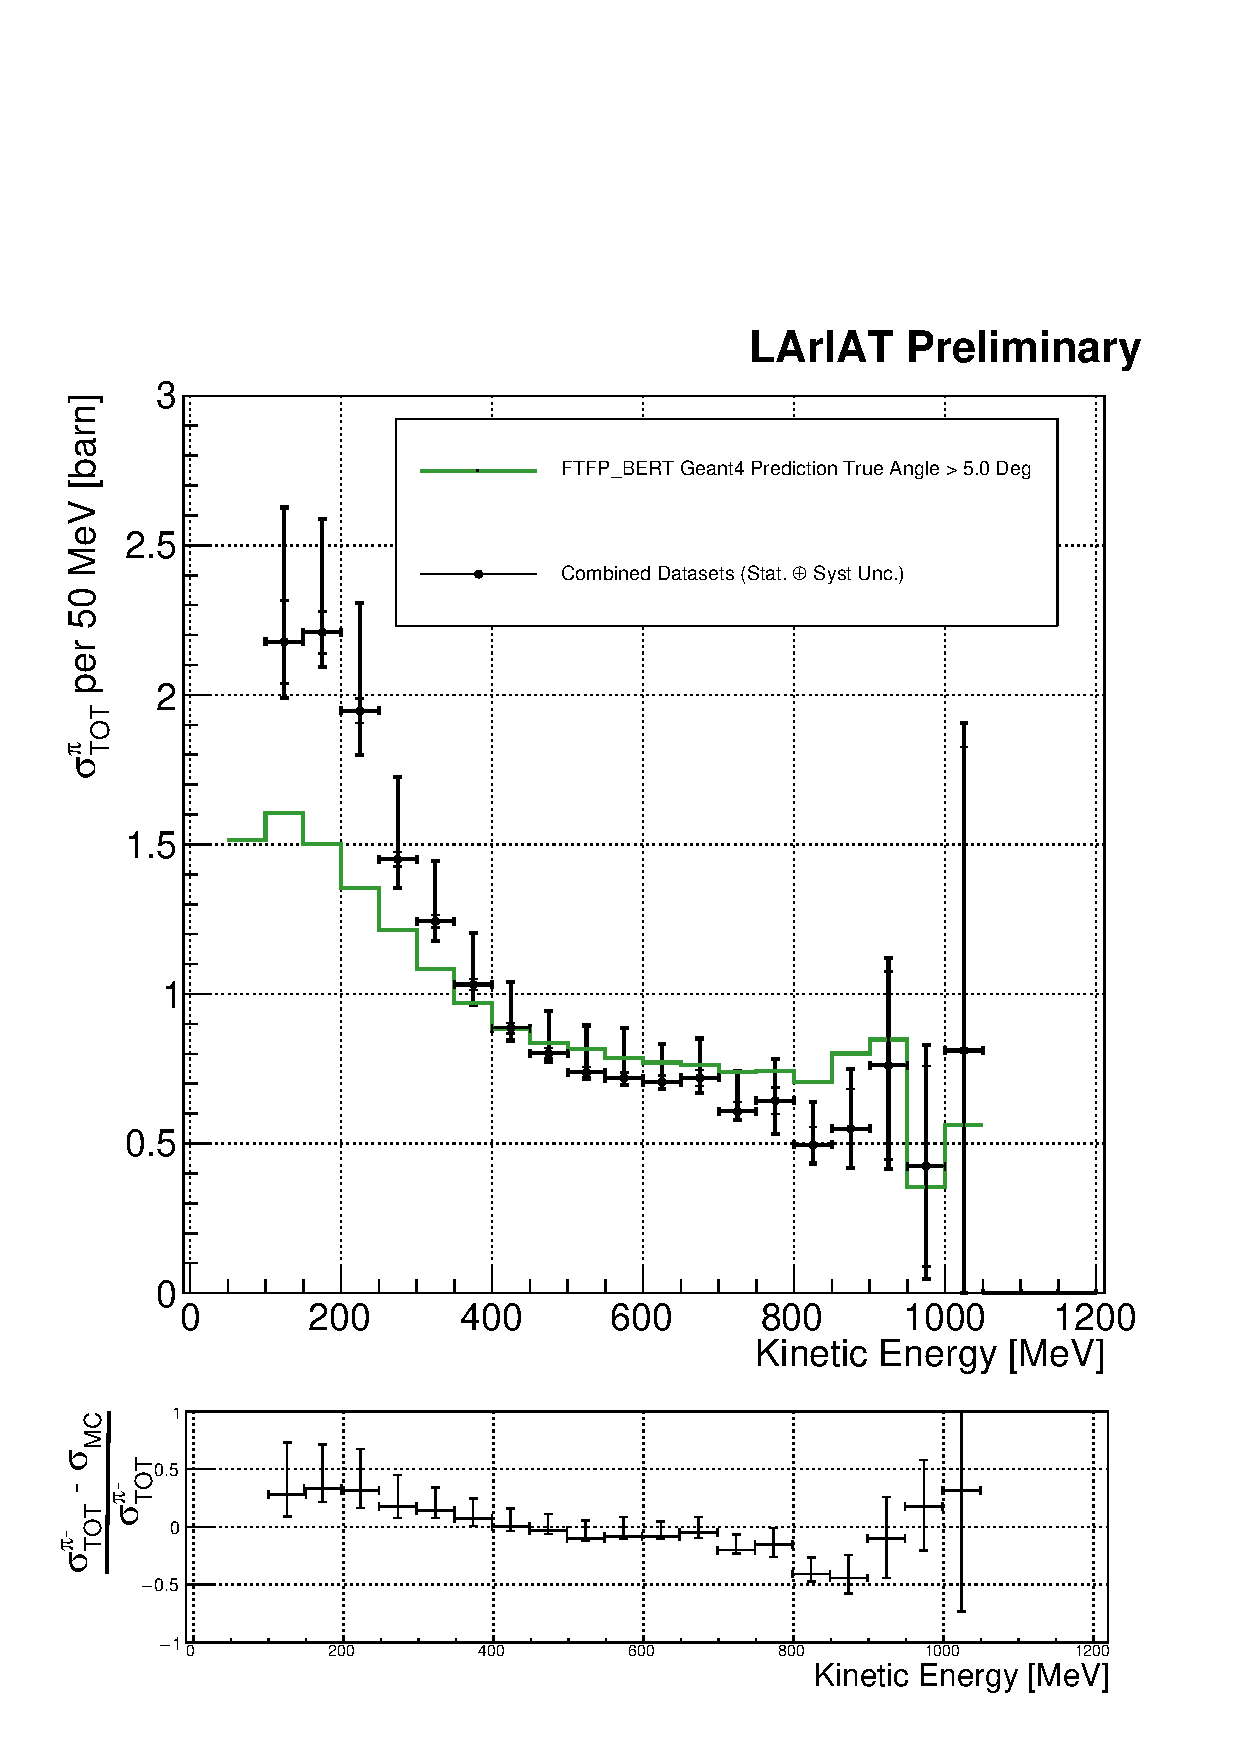
\includegraphics[width =0.4\textwidth ]{TheRealMoneyPlot}
\caption{\label{fig:epsart} Top: ($\pi^-$-Ar) total hadronic cross section for  scattering angles greater than 5$^\circ$ measured in the combined sample, statistical uncertainty and systematic uncertainty in black. The Geant4 prediction for the total hadronic cross section for angle scattering greater than 5$^\circ$ is displayed in green. Bottom: Relative difference between the measured cross section and the Geant4 prediction. }
\end{figure}

\begin{table*}
\caption{\label{tab:XSsummary} Results summary. }
\begin{ruledtabular}
\begin{tabular}{ccccccc}
$[E^{kin}_{\text{MIN}}, E^{kin}_{\text{MAX}}]$ & $\sigma_{\text{TOT}}$ & Stat $\bigoplus$ Syst  & $N^{ \text{Data}}_{ \text{Int}} - B^{ \text{Int}}$
& $N^{ \text{Data}}_{ \text{Inc}} - B^{ \text{Inc}}$ & $ \epsilon^{\text{Int}} $ & $\epsilon^{\text{Inc}}$ \\ 
(MeV)& (Barn)& Uncertainty (Barn) & & & \\\hline
& & & & & \\
 $[100,150]$ &1&+20/-10 & & & & \\
\end{tabular}
\end{ruledtabular}
\end{table*}



\begin{comment}
This sample document demonstrates proper use of REV\TeX~4 (and
\LaTeXe) in mansucripts prepared for submission to APS
journals. Further information can be found in the REV\TeX~4
documentation included in the distribution or available at
\url{http://publish.aps.org/revtex4/}.

When commands are referred to in this example file, they are always
shown with their required arguments, using normal \TeX{} format. In
this format, \verb+#1+, \verb+#2+, etc. stand for required
author-supplied arguments to commands. For example, in
\verb+\section{#1}+ the \verb+#1+ stands for the title text of the
author's section heading, and in \verb+\title{#1}+ the \verb+#1+
stands for the title text of the paper.

Line breaks in section headings at all levels can be introduced using
\textbackslash\textbackslash. A blank input line tells \TeX\ that the
paragraph has ended. Note that top-level section headings are
automatically uppercased. If a specific letter or word should appear in
lowercase instead, you must escape it using \verb+\lowercase{#1}+ as
in the word ``via'' above.

%\subsection{\label{sec:level2}Second-level heading: Formatting}
% subsections are not used for PRL papers

This file may be formatted in both the \texttt{preprint} and
\texttt{twocolumn} styles. \texttt{twocolumn} format may be used to
mimic final journal output. Either format may be used for submission
purposes; however, for peer review and production, APS will format the
article using the \texttt{preprint} class option. Hence, it is
essential that authors check that their manuscripts format acceptably
under \texttt{preprint}. Manuscripts submitted to APS that do not
format correctly under the \texttt{preprint} option may be delayed in
both the editorial and production processes.

The \texttt{widetext} environment will make the text the width of the
full page.  The width-changing commands only take effect in \texttt{twocolumn}
formatting. It has no effect if \texttt{preprint} formatting is chosen
instead.

To cite bibliography entries, use the \verb+\cite{#1}+ command. Most
journal styles will display the corresponding number(s) in square
brackets: \cite{d0det}. To avoid the square brackets, use
\verb+\onlinecite{#1}+: Refs.~\onlinecite{d0det} and
\onlinecite{geant,pythia}. REV\TeX\ ``collapses'' lists of
consecutive reference numbers where possible. We now cite everyone
together \cite{geant, pythia, cteq}, and once again
(Refs.~\onlinecite{geant, pythia, cteq}). Note that the references
were also sorted into the correct numerical order as well.

Footnotes are produced using the \verb+\footnote{#1}+ command. Most
APS journal styles put footnotes into the bibliography. REV\TeX~4 does
this as well, but instead of interleaving the footnotes with the
references, they are listed at the end of the references. Because the correct
numbering of the footnotes must occur after the numbering of the
references, an extra pass of \LaTeX\ is required in order to get the
numbering correct.


Inline math may be typeset using the \verb+$+ delimiters. Bold math
symbols may be achieved using the \verb+bm+ package and the
\verb+\bm{#1}+ command it supplies. For instance, a bold $\alpha$ can
be typeset as \verb+$\bm{\alpha}$+ giving $\bm{\alpha}$. Fraktur and
Blackboard (or open face or double struck) characters should be
typeset using the \verb+\mathfrak{#1}+ and \verb+\mathbb{#1}+ commands
respectively. Both are supplied by the \texttt{amssymb} package. For
example, \verb+$\mathbb{R}$+ gives $\mathbb{R}$ and
\verb+$\mathfrak{G}$+ gives $\mathfrak{G}$

In \LaTeX\ there are many different ways to display equations, and a
few preferred ways are noted below. Displayed math will center by
default. Use the class option \verb+fleqn+ to flush equations left.

Below we have numbered single-line equations; this is the most common
type of equation in \textit{Physical Review}:
\begin{eqnarray}
\chi_+(p)\alt{\bf [}2|{\bf p}|(|{\bf p}|+p_z){\bf ]}^{-1/2}
\left(
\begin{array}{c}
|{\bf p}|+p_z\\
px+ip_y
\end{array}\right)\;,
\\
\left\{%
 \openone234567890abc123\alpha\beta\gamma\delta1234556\alpha\beta
 \frac{1\sum^{a}_{b}}{A^2}%
\right\}%
\label{eq:one}.
\end{eqnarray}
Note the open one in Eq.~(\ref{eq:one}).

Not all numbered equations will fit within a narrow column this
way. The equation number will move down automatically if it cannot fit
on the same line with a one-line equation:
\begin{equation}
\left\{
 ab12345678abc123456abcdef\alpha\beta\gamma\delta1234556\alpha\beta
 \frac{1\sum^{a}_{b}}{A^2}%
\right\}.
\end{equation}

When the \verb+\label{#1}+ command is used [cf. input for
Eq.~(\ref{eq:one})], the equation can be referred to in text without
knowing the equation number that \TeX\ will assign to it. Just
use \verb+\ref{#1}+, where \verb+#1+ is the same name that used in
the \verb+\label{#1}+ command.

Unnumbered single-line equations can be typeset
using the \verb+\[+, \verb+\]+ format:
\[g^+g^+ \rightarrow g^+g^+g^+g^+ \dots ~,~~q^+q^+\rightarrow
q^+g^+g^+ \dots ~. \]


Figures may be inserted by using either the \texttt{graphics} or
\texttt{graphicx} packages. These packages both define the
\verb+\includegraphics{#1}+ command, but they differ in how optional
arguments for specifying the orientation, scaling, and translation of the
figure. Fig.~\ref{fig:epsart} shows a figure that is small enough to
fit in a single column. It is embedded using the \texttt{figure}
environment which provides both the caption and the imports the figure
file.

\begin{figure}
\includegraphics[scale=0.8]{TheRealMoneyPlot.ps}
\caption{\label{fig:epsart} A figure caption. The figure captions are
automatically numbered.}
\end{figure}

Fig.~\ref{fig:wide} is a figure that is too wide for a single column,
so instead the \texttt{figure*} environment has been used.
\begin{figure*}
%\includegraphics{fig_2.ps}% Here is how to import EPS art
\caption{\label{fig:wide}Use the figure* environment to get a wide
figure that spans the page in \texttt{twocolumn} formatting.}
\end{figure*}


The heart of any table is the \texttt{tabular} environment which gives
the rows of the tables. Each row consists of column entries separated
by \verb+&+'s and terminates with \textbackslash\textbackslash. The
required argument for the \texttt{tabular} environment
specifies how data are displayed in the columns. For instance, entries
may be centered, left-justified, right-justified, aligned on a decimal
point. Extra column-spacing may be be specified as well, although
REV\TeX~4 sets this spacing so that the columns fill the width of the
table. Horizontal rules are typeset using the \verb+\hline+
command. The doubled (or Scotch) rules that appear at the top and
bottom of a table can be achieved enclosing the \texttt{tabular}
environment within a \texttt{ruledtabular} environment. Rows whose
columns span multiple columns can be typeset using the
\verb+\multicolumn{#1}{#2}{#3}+ command (for example, see the first
row of Table~\ref{tab:table3}).

Tables~\ref{tab:table1}-\ref{tab:table4} show various effects. Tables
that fit in a narrow column are contained in a \texttt{table}
environment. Table~\ref{tab:table3} is a wide table set with the
\texttt{table*} environment. Long tables may need to break across
pages. The most straightforward way to accomplish this is to specify
the \verb+[H]+ float placement on the \texttt{table} or
\texttt{table*} environment. However, the standard \LaTeXe\ package
\texttt{longtable} will give more control over how tables break and
will allow headers and footers to be specified for each page of the
table. A simple example of the use of \texttt{longtable} can be found
in the file \texttt{summary.tex} that is included with the REV\TeX~4
distribution.

There are two methods for setting footnotes within a table (these
footnotes will be displayed directly below the table rather than at
the bottom of the page or in the bibliography). The easiest
and preferred method is just to use the \verb+\footnote{#1}+
command. This will automatically enumerate the footnotes with
lowercase roman letters. However, it is sometimes necessary to have
multiple entries in the table share the same footnote. In this case,
there is no choice but to manually create the footnotes using
\verb+\footnotemark[#1]+ and \verb+\footnotetext[#1]{#2}+.
\texttt{\#1} is a numeric value. Each time the same value for
\texttt{\#1} is used, the same mark is produced in the table. The
\verb+\footnotetext[#1]{#2}+ commands are placed after the \texttt{tabular}
environment. Examine the \LaTeX\ source and output for
Tables~\ref{tab:table1} and \ref{tab:table2} for examples.

\begin{table}
\caption{\label{tab:table1}This is a narrow table which fits into a
narrow column when using \texttt{twocolumn} formatting. Note that
REV\TeX~4 adjusts the intercolumn spacing so that the table fills the
entire width of the column. Table captions are numbered
automatically. This table illustrates left-aligned, centered, and
right-aligned columns.  }
\begin{ruledtabular}
\begin{tabular}{lcr}
Left\footnote{Note a.}&Centered\footnote{Note b.}&Right\\
\hline
1 & 2 & 3\\
10 & 20 & 30\\
100 & 200 & 300\\
\end{tabular}
\end{ruledtabular}
\end{table}

\begin{table}
\caption{\label{tab:table2}A table with more columns still fits
properly in a column. Note that several entries share the same
footnote. Inspect the \LaTeX\ input for this table to see
exactly how it is done.}
\begin{ruledtabular}
\begin{tabular}{cccccccc}
 &$r_c$ (\AA)&$r_0$ (\AA)&$\kappa r_0$&
 &$r_c$ (\AA) &$r_0$ (\AA)&$\kappa r_0$\\
\hline
Cu& 0.800 & 14.10 & 2.550 &Sn\footnotemark[1]
& 0.680 & 1.870 & 3.700 \\
Ag& 0.990 & 15.90 & 2.710 &Pb\footnotemark[2]
& 0.450 & 1.930 & 3.760 \\
Au& 1.150 & 15.90 & 2.710 &Ca\footnotemark[3]
& 0.750 & 2.170 & 3.560 \\
Mg& 0.490 & 17.60 & 3.200 &Sr\footnotemark[4]
& 0.900 & 2.370 & 3.720 \\
Zn& 0.300 & 15.20 & 2.970 &Li\footnotemark[2]
& 0.380 & 1.730 & 2.830 \\
Cd& 0.530 & 17.10 & 3.160 &Na\footnotemark[5]
& 0.760 & 2.110 & 3.120 \\
Hg& 0.550 & 17.80 & 3.220 &K\footnotemark[5]
&  1.120 & 2.620 & 3.480 \\
Al& 0.230 & 15.80 & 3.240 &Rb\footnotemark[3]
& 1.330 & 2.800 & 3.590 \\
Ga& 0.310 & 16.70 & 3.330 &Cs\footnotemark[4]
& 1.420 & 3.030 & 3.740 \\
In& 0.460 & 18.40 & 3.500 &Ba\footnotemark[5]
& 0.960 & 2.460 & 3.780 \\
Tl& 0.480 & 18.90 & 3.550 & & & & \\
\end{tabular}
\end{ruledtabular}
\footnotetext[1]{Here's the first, from Ref.~\onlinecite{pdg}.}
\footnotetext[2]{Here's the second.}
\footnotetext[3]{Here's the third.}
\footnotetext[4]{Here's the fourth.}
\footnotetext[5]{And etc.}
\end{table}

\begin{table*}
\caption{\label{tab:table3}This is a wide table that spans the page
width in \texttt{twocolumn} mode. It is formatted using the
\texttt{table*} environment. It also demonstates the use of
\textbackslash\texttt{multicolumn} in rows with entries that span
more than one column.}
\begin{ruledtabular}
\begin{tabular}{ccccc}
 &\multicolumn{2}{c}{$D_{4h}^1$}&\multicolumn{2}{c}{$D_{4h}^5$}\\
 Ion&1st alternative&2nd alternative&lst alternative
&2nd alternative\\ \hline
 K&$(2e)+(2f)$&$(4i)$ &$(2c)+(2d)$&$(4f)$ \\
 Mn&$(2g)$\footnote{The $z$ parameter of these positions is $z\sim\frac{1}{4}$.}
 &$(a)+(b)+(c)+(d)$&$(4e)$&$(2a)+(2b)$\\
 Cl&$(a)+(b)+(c)+(d)$&$(2g)$\footnotemark[1]
 &$(4e)^{\text{a}}$\\
 He&$(8r)^{\text{a}}$&$(4j)^{\text{a}}$&$(4g)^{\text{a}}$\\
 Ag& &$(4k)^{\text{a}}$& &$(4h)^{\text{a}}$\\
\end{tabular}
\end{ruledtabular}
\end{table*}

\begin{table}
\caption{\label{tab:table4}Numbers in columns Three--Five have been
aligned by using the ``d'' column specifier (requires the
\texttt{dcolumn} package). Non-numeric entries (those entries without
a ``.'') in a ``d'' column are aligned on the decimal point. Use the
``D'' specifier for more complex layouts. }
\begin{ruledtabular}
\begin{tabular}{ccddd}
One&Two&\mbox{Three}&\mbox{Four}&\mbox{Five}\\
\hline
one&two&\mbox{three}&\mbox{four}&\mbox{five}\\
He&2& 2.77234 & 45672. & 0.69 \\
C\footnote{Some tables require footnotes.}
  &C\footnote{Some tables need more than one footnote.}
  & 12537.64 & 37.66345 & 86.37 \\
\end{tabular}
\end{ruledtabular}
\end{table}



\textit{Physical Review} style requires that the initial citation of
figures or tables be in numerical order in text, so don't cite
Fig.~\ref{fig:wide} until Fig.~\ref{fig:epsart} has been cited.

%%%%%%%%%%%%%%


%Historic measurements of hadronic cross sections are performed on thin targets [\textcolor{red}{A CIT is needed here}]. At their core, these experiments consists in shooting a beam of particles with a known flux on a thin slab of material and recording the outgoing flux, under the assumption that the target centers are uniformly distributed in the material and that no center of interaction sits in front of another. 


%The thin target approximation is valid if the interaction length of the considered process is significantly longer than the width of the target, i.e $\lambda_{\text{Int}} \gg \delta X$.

%Equation \ref{eq:thinTargetXS},
%\begin{equation}
%P_{\text{Surv}} = e^{-\sigma_{\text{TOT}}\text{ } n \text{ }\delta X} = 1- P_{\text{Int}}  = 1 - \frac{N_{\text{Int}}}{N_{\text{Inc}}} 
%\label{eq:thinTargetXS}
%\end{equation}
% relates the probability that a particle survives a target to the total hadronic cross section, $\sigma_{\text{TOT}}$, the density of the target centers, $n$,  and  the thickness of the target  along the incident hadron direction, $\delta X$. The survival probability can be expressed in terms of the interaction probability $P_{\text{Int}}$, represented by ratio between the number of particles interacting in the thin target $N_{\text{Int}}$ and the number of incident particles $N_{\text{Inc}}$. In the thin target approximation,  a simple proportionality relationship between the cross section and the interaction probability is found by Taylor expanding the exponential function:
% \begin{equation}
% \sigma_{\text{TOT}}  = \frac{1}{n \text{ }\delta X}\frac{N_{\text{Int}}}{N_{\text{Inc}}}.
%\label{eq:thinTargetXSSolved}
%\end{equation}

%Since the expected interaction length of pions in liquid argon is of the order of $\lambda_{\text{Int}} \sim 50$ cm [\textcolor{red}{A CIT is needed here}], we cannot treat the LArIAT TPC, with its 90 cm of length,  as a thin target. However, the granularity of the LArIAT LArTPC allows us to assess the presence of a pion and to measure its kinetic energy approximately every 4.7~mm along its trajectory in the detector's active volume. We can thus treat the argon volume as a sequence of many adjacent thin targets, recovering the thin target approximation in each slice of argon. 


%\begin{figure}
%  \centering  
%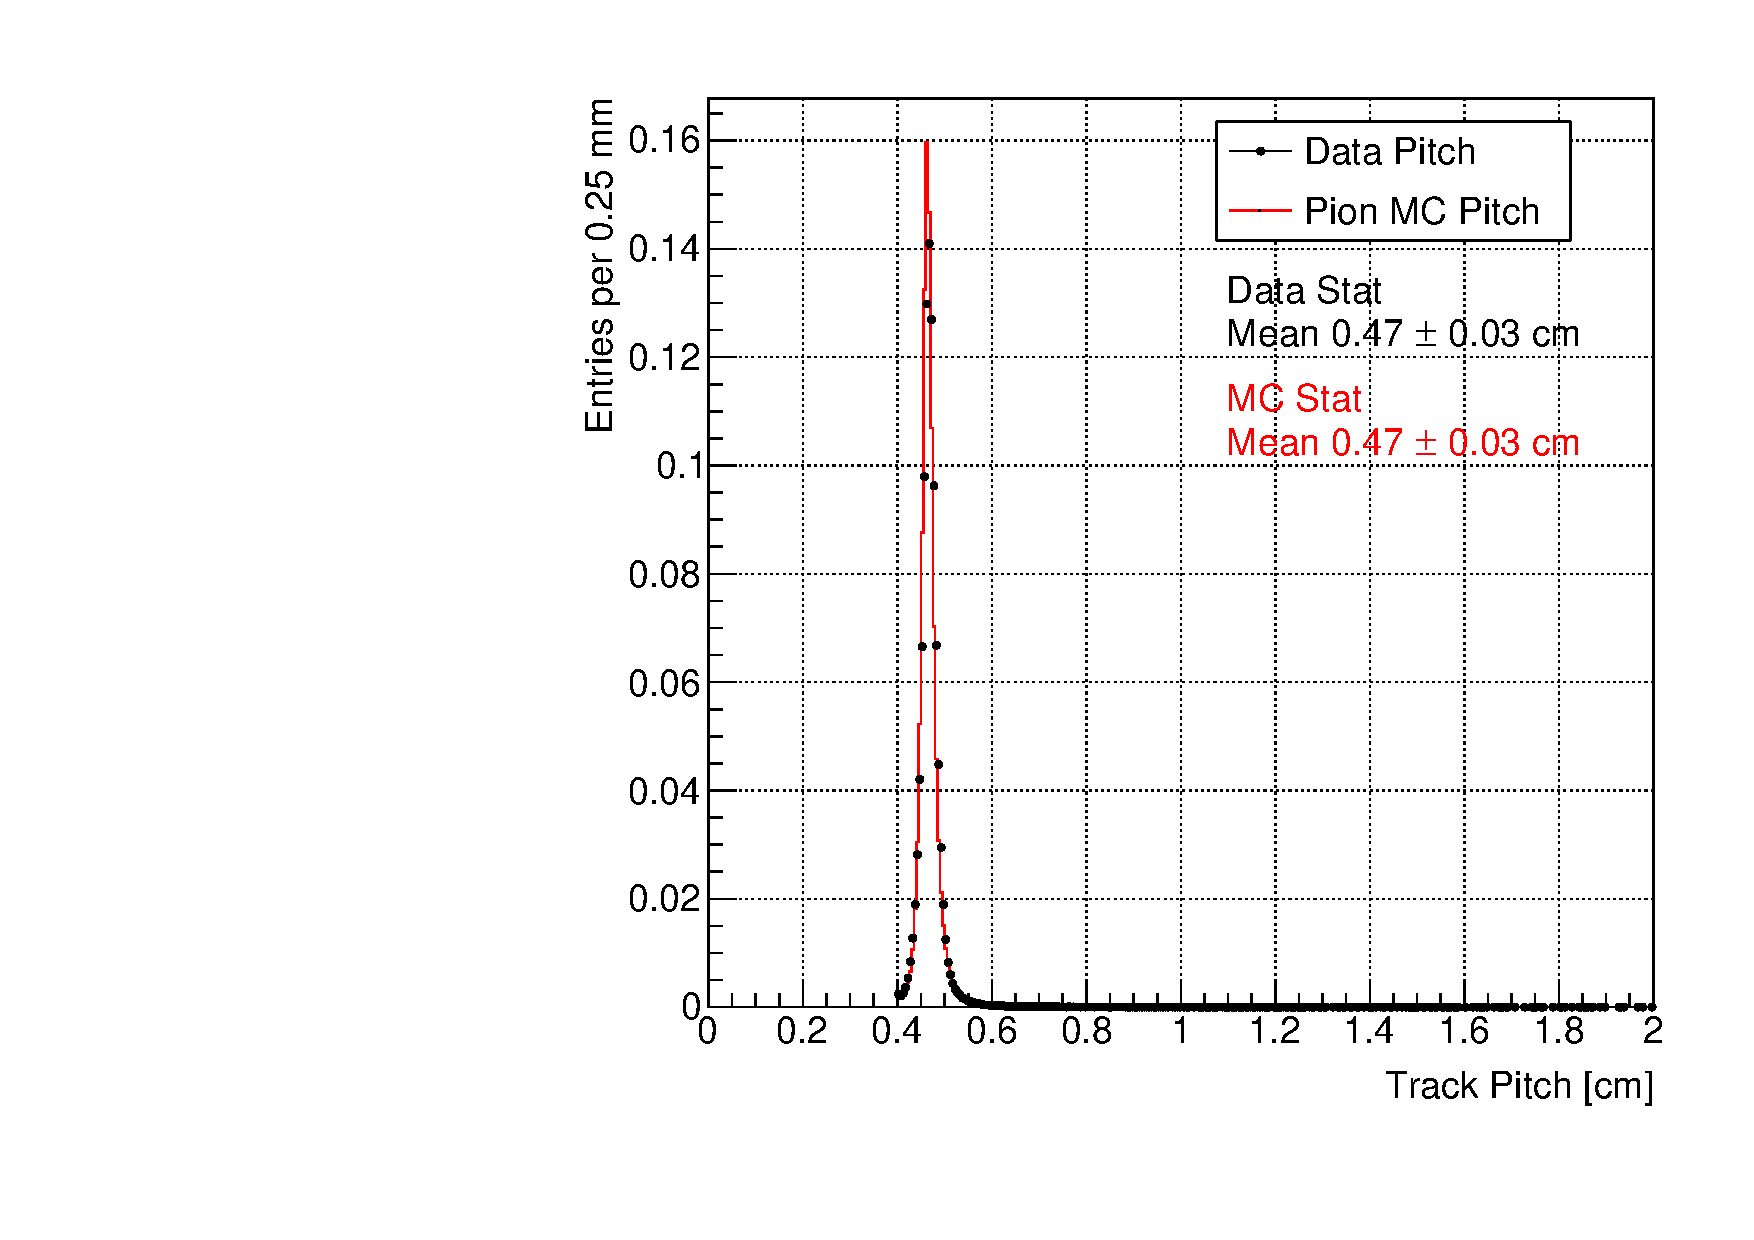
\includegraphics[width=0.8\textwidth]{PitchPi}
%\caption{Representation of sliced LAr Volume.}
%\label{fig:TPCGran}
%\end{figure}


\end{comment}

\input acknowledgement.tex   % input acknowledgement

\begin{thebibliography}{99}

  \bibitem{LArIATDet}
    Standard LArIAT detector reference:  \\
R. Acciarri {\sl et al.} (LArIAT Collaboration),
hopefully we'll have one soon.

 \end{thebibliography}

\end{document}
%
% ****** End of file template.aps ******
